\documentclass[12pt]{article}
\usepackage{fancyhdr}
\usepackage{amsmath,amsfonts,enumerate}
\usepackage{color,graphicx}
\usepackage{tikz}
\usepackage{pgfplots}
\usepackage{listings}
\usepackage{algorithm}
\usepackage{algorithmic}
\usetikzlibrary{arrows,positioning,shapes,calc,matrix}
\pagestyle{fancy}

% Define colors for answers
\definecolor{answercolor}{RGB}{0,100,0}
\definecolor{explanationcolor}{RGB}{0,0,139}

% Custom commands for answers
\newcommand{\answer}[1]{{\color{answercolor}\textbf{Answer:} #1}}
\newcommand{\explanation}[1]{{\color{explanationcolor}#1}}

%%%%%%%%%%%%%%%%%%%%%%%%%%%%%%%%%%%%%%%%%%%%%%%%%
% Course customization based on university sources
%%%%%%%%%%%%%%%%%%%%%%%%%%%%%%%%%%%%%%%%%%%%%%%%%
\newcommand{\masunitnumber}{CENG 403}
\newcommand{\examdate}{January 2025}
\newcommand{\academicyear}{2024-2025}
\newcommand{\semester}{I}
\newcommand{\coursename}{Deep Learning - CNN Architecture Design \& Transfer Learning (University Sources) - ANSWERED}
\newcommand{\numberofhours}{3}
%%%%%%%%%%%%%%%%%%%%%%%%%%%%%%%%%%%%%%%%%%%%%%%%%
% CUSTOM SPACING COMMANDS FOR ANSWER SPACES
%%%%%%%%%%%%%%%%%%%%%%%%%%%%%%%%%%%%%%%%%%%%%%%%%
\newcommand{\answerspace}[1]{\vspace{#1}}
\newcommand{\questionspace}{\vspace{3cm}}        
\newcommand{\subquestionspace}{\vspace{2.5cm}}   
\newcommand{\shortanswer}{\vspace{2cm}}          
\newcommand{\mediumanswer}{\vspace{3cm}}         
\newcommand{\longanswer}{\vspace{4cm}}           
\newcommand{\journalspace}{\vspace{4.5cm}}       
\newcommand{\codespace}{\vspace{5cm}}            
%%%%%%%%%%%%%%%%%%%%%%%%%%%%%%%%%%%%%%%%%%%%%%%%%
% Header setup
%%%%%%%%%%%%%%%%%%%%%%%%%%%%%%%%%%%%%%%%%%%%%%%%%
\lhead{}
\rhead{}
\chead{{\bf MIDDLE EAST TECHNICAL UNIVERSITY}}
\lfoot{}
\rfoot{}
\cfoot{}
\begin{document}
\setlength{\headsep}{5truemm}
\setlength{\headheight}{14.5truemm}
\setlength{\voffset}{-0.45truein}
\renewcommand{\headrulewidth}{0.0pt}
\begin{center}
SEMESTER \semester\ EXAMINATION \academicyear
\end{center}
\begin{center}
{\bf \masunitnumber\ -- \coursename}
\end{center}
\vspace{20truemm}
\noindent \examdate\hspace{45truemm} TIME ALLOWED: \numberofhours\ HOURS
\vspace{19truemm}
\hrule
\vspace{19truemm}
\noindent\underline{INSTRUCTIONS TO CANDIDATES}
\vspace{8truemm}
%%%%%%%%%%%%%%%%%%%%%%%%%%%%%%%%%%%%%%%%%%%%%%%%%%%%%%
% Instructions based on university standards
%%%%%%%%%%%%%%%%%%%%%%%%%%%%%%%%%%%%%%%%%%%%%%%%%%%%%%
\begin{enumerate}
\item This examination paper contains {\bf SEVEN (7)} questions and comprises 
{\bf TEN (10)} printed pages.
\item Answer all questions. 
The marks for each question are indicated at the beginning of each question.
\item Answer each question beginning on a {\bf FRESH} page of the answer book.
\item This {\bf IS NOT an OPEN BOOK} exam.
\item Show all mathematical derivations clearly with proper notation.
\item For architectural diagrams, draw clear and labeled components.
\item Calculate all requested parameters and show intermediate steps.
\item Explain computational complexity where requested.
\end{enumerate}
%%%%%%%%%%%%%%%%%%%%%%%%%%%%%%%%%%%%%%%%%%%%%%%%%
% New page for questions
%%%%%%%%%%%%%%%%%%%%%%%%%%%%%%%%%%%%%%%%%%%%%%%%%
\newpage
\lhead{}
\rhead{\masunitnumber}
\chead{}
\lfoot{}
\cfoot{\thepage}
\rfoot{}
\setlength{\footskip}{45pt}
%%%%%%%%%%%%%%%%%%%%%%%%%%%%%%%%%%%%%%%%%%%%%%%%%%
% EXAM QUESTIONS BASED ON UNIVERSITY SOURCES
%%%%%%%%%%%%%%%%%%%%%%%%%%%%%%%%%%%%%%%%%%%%%%%%%%

\paragraph{Question 1. Position-Sensitive Convolution Mathematical Analysis}{{\hfill (25 marks)}}\\
Based on Stanford CS231n and university computer vision course materials.

\begin{enumerate}[(a)]
    \item Formulate position-sensitive convolution mathematically. Given input $X \in \mathbb{R}^{H \times W \times C}$, derive the augmented input formulation: \hfill (10 marks)
    \begin{itemize}
        \item Show $X_{aug}(i,j) = [X(i,j), \frac{i}{H}, \frac{j}{W}]$ where coordinates are normalized to [0,1]
        \item Explain why vanilla convolution fails for position estimation tasks
        \item Calculate the increased computational cost: memory and FLOPs for coordinate channels
    \end{itemize}

    \answer{Position-sensitive convolution extends regular convolution by incorporating spatial coordinate information directly into the input representation.}
    
    \explanation{
    \textbf{Mathematical Formulation:}
    
    For input $X \in \mathbb{R}^{H \times W \times C}$, the augmented input becomes:
    $$X_{aug}(i,j) = [X(i,j), \frac{i}{H}, \frac{j}{W}] \in \mathbb{R}^{C+2}$$
    
    where:
    \begin{itemize}
        \item $X(i,j) \in \mathbb{R}^C$ is the original feature vector at position $(i,j)$
        \item $\frac{i}{H}, \frac{j}{W}$ are normalized coordinates in $[0,1]$
        \item The augmented feature dimension becomes $C+2$
    \end{itemize}
    
    \textbf{Why Vanilla Convolution Fails for Position Estimation:}
    
    Regular convolution is translation equivariant: if input shifts by $(\Delta i, \Delta j)$, output shifts by the same amount. This property is problematic for position estimation because:
    \begin{itemize}
        \item The network cannot distinguish between identical patterns at different locations
        \item Pooling operations further reduce spatial information
        \item The network learns to ignore absolute position, focusing only on local patterns
    \end{itemize}
    
    \textbf{Computational Cost Analysis:}
    
    Memory increase: $(C+2)/C = 1 + \frac{2}{C}$ factor increase
    
    For typical CNN with $C=256$: $1 + \frac{2}{256} = 1.0078$ (0.78\% increase)
    
    FLOPs increase: Each convolution kernel now processes $C+2$ channels instead of $C$
    
    For kernel size $k \times k$: FLOPs increase by factor $(C+2)/C$
    
    The computational overhead is minimal (typically $<1\%$) while providing significant capability for position-aware tasks.
    }
    
    \item Analyze the mathematical foundation of pooling invariances. For max pooling with receptive field $R$ and stride $s$: \hfill (10 marks)
    \begin{itemize}
        \item Derive translation invariance: if $X'(i,j) = X(i+\delta, j+\delta)$ where $|\delta| < s$, show when $\text{MaxPool}(X') = \text{MaxPool}(X)$
        \item Calculate the exact translation tolerance for different pooling configurations
        \item Compare mathematical properties of max pooling vs. average pooling for invariance
    \end{itemize}
    
    \answer{Max pooling provides approximate translation invariance within the stride distance, but this invariance breaks down for larger translations.}
    
    \explanation{
    \textbf{Translation Invariance Derivation:}
    
    For max pooling with receptive field $R \times R$ and stride $s$:
    
    Original pooling: $\text{MaxPool}(X)_{i,j} = \max_{u,v \in R_{i,j}} X(u,v)$
    
    Translated input: $X'(u,v) = X(u+\delta, v+\delta)$ where $|\delta| < s$
    
    For small translations ($|\delta| < s$), the receptive field $R_{i,j}$ still covers most of the same values:
    $$\text{MaxPool}(X')_{i,j} = \max_{u,v \in R_{i,j}} X(u+\delta, v+\delta) = \max_{u,v \in R'_{i,j}} X(u,v)$$
    
    where $R'_{i,j}$ is the shifted receptive field.
    
    \textbf{Exact Translation Tolerance:}
    
    \begin{itemize}
        \item For $2 \times 2$ pooling with stride 2: Perfect invariance for $|\delta| < 1$
        \item For $3 \times 3$ pooling with stride 2: Partial invariance for $|\delta| < 2$, perfect for $|\delta| < 1$
        \item General case: Tolerance decreases as $\frac{R-s}{R}$ of the receptive field overlaps
    \end{itemize}
    
    \textbf{Max vs. Average Pooling Comparison:}
    
    Max Pooling:
    \begin{itemize}
        \item Provides stronger invariance to small translations
        \item Non-linear operation: $\max(a+\epsilon, b+\epsilon) = \max(a,b) + \epsilon$ only if the same element remains maximum
        \item Sensitive to outliers but robust to noise in non-maximum elements
    \end{itemize}
    
    Average Pooling:
    \begin{itemize}
        \item Linear operation: $\frac{1}{R^2}\sum(X + \epsilon) = \frac{1}{R^2}\sum X + \epsilon$
        \item More stable but less invariant to small translations
        \item Preserves more information but reduces discriminative power
    \end{itemize}
    }
    
    \item Design an experimental validation for position-sensitive convolution effectiveness: \hfill (5 marks)
    \begin{itemize}
        \item Propose synthetic datasets for controlled position estimation evaluation
        \item Define quantitative metrics for position accuracy assessment
        \item Statistical significance testing for performance comparison
    \end{itemize}
    
    \answer{A controlled experimental setup using synthetic datasets with known ground truth positions allows precise evaluation of position-sensitive convolution effectiveness.}
    
    \explanation{
    \textbf{Synthetic Dataset Design:}
    
    \begin{enumerate}
        \item \textbf{Geometric Patterns Dataset:} Simple shapes (circles, squares, triangles) at random positions in $224 \times 224$ images
        \item \textbf{MNIST Position Dataset:} MNIST digits placed at specific coordinates with task to predict $(x,y)$ location
        \item \textbf{Multi-object Scenes:} Multiple objects with varying scales and positions
    \end{enumerate}
    
    \textbf{Quantitative Metrics:}
    
    \begin{itemize}
        \item \textbf{Mean Absolute Error (MAE):} $\text{MAE} = \frac{1}{N}\sum_{i=1}^N ||\hat{p}_i - p_i||_2$ where $p_i$ is true position, $\hat{p}_i$ is predicted
        \item \textbf{Pixel Accuracy:} Percentage of predictions within $k$ pixels of ground truth
        \item \textbf{Normalized Error:} $\frac{||\hat{p} - p||_2}{\text{image\_diagonal}}$ for scale-invariant comparison
    \end{itemize}
    
    \textbf{Statistical Testing:}
    
    Use paired t-test comparing position-sensitive CNN vs. vanilla CNN:
    $$t = \frac{\bar{d} - 0}{s_d/\sqrt{n}}$$
    where $d_i = \text{Error}_{\text{vanilla},i} - \text{Error}_{\text{pos-sensitive},i}$
    
    Significance level: $\alpha = 0.05$ with Bonferroni correction for multiple comparisons.
    }
\end{enumerate}

\newpage
\paragraph{Question 2. Global Average Pooling vs. Fully Connected Layers}{{\hfill (28 marks)}}\\
Based on MIT 6.034 and university machine learning course materials.

\begin{enumerate}[(a)]
    \item Analyze the parameter explosion problem in fully connected layers. For a CNN with final feature map of size $H \times W \times C$ and $N$ output classes: \hfill (12 marks)
    \begin{itemize}
        \item Calculate exact parameter count for FC approach: $(H \times W \times C) \times N + N$
        \item Show GAP parameter count: $C \times N + N$
        \item For AlexNet (6×6×256 → 4096 → 4096 → 1000), compute parameter reduction percentage
        \item Analyze memory footprint implications for training and inference
    \end{itemize}
    
    \answer{Global Average Pooling dramatically reduces parameters compared to fully connected layers while maintaining representational capability.}
    
    \explanation{
    \textbf{Parameter Count Analysis:}
    
    FC Approach:
    \begin{itemize}
        \item First FC layer: $(H \times W \times C) \times N$ weights + $N$ biases
        \item Total: $(H \times W \times C + 1) \times N$ parameters
    \end{itemize}
    
    GAP Approach:
    \begin{itemize}
        \item GAP operation: 0 parameters (just averaging)
        \item Classification layer: $C \times N$ weights + $N$ biases
        \item Total: $(C + 1) \times N$ parameters
    \end{itemize}
    
    \textbf{AlexNet Calculation:}
    
    Original AlexNet FC layers:
    \begin{itemize}
        \item FC1: $6 \times 6 \times 256 \times 4096 = 37,748,736$ parameters
        \item FC2: $4096 \times 4096 = 16,777,216$ parameters  
        \item FC3: $4096 \times 1000 = 4,096,000$ parameters
        \item Total FC parameters: $58,621,952$
    \end{itemize}
    
    GAP alternative:
    \begin{itemize}
        \item Classification layer: $256 \times 1000 = 256,000$ parameters
        \item Reduction: $\frac{58,621,952 - 256,000}{58,621,952} = 99.56\%$ reduction
    \end{itemize}
    
    \textbf{Memory Footprint Analysis:}
    
    Training Memory (per sample):
    \begin{itemize}
        \item FC: Store activations for $(H \times W \times C) + N$ neurons
        \item GAP: Store activations for $C + N$ neurons
        \item Gradient storage: Proportional to parameter count
    \end{itemize}
    
    Inference Memory:
    \begin{itemize}
        \item FC: Model size dominated by FC weights
        \item GAP: Dramatically smaller model size enables mobile deployment
    \end{itemize}
    }
    
    \item Prove the mathematical equivalence between GAP and specialized channel learning: \hfill (10 marks)
    \begin{itemize}
        \item Given feature map $F_k(x,y)$ for channel $k$, show GAP output: $g_k = \frac{1}{HW}\sum_{x,y} F_k(x,y)$
        \item Derive how network learns to optimize: $\max_{F_k} \sum_k w_{k,c} \cdot g_k$ for class $c$
        \item Explain why this forces $F_k$ to become confidence maps for specific objects
        \item Mathematical justification for why "one fully connected layer is sufficient"
    \end{itemize}
    
    \answer{GAP creates an inductive bias that forces each channel to specialize as a confidence map for specific semantic concepts.}
    
    \explanation{
    \textbf{GAP Mathematical Formulation:}
    
    For feature map $F_k(x,y)$ in channel $k$:
    $$g_k = \frac{1}{HW}\sum_{x=1}^H \sum_{y=1}^W F_k(x,y)$$
    
    This transforms spatial feature maps into a single scalar per channel.
    
    \textbf{Optimization Objective:}
    
    The network learns to maximize the probability of correct class $c$:
    $$P(y=c|x) = \text{softmax}\left(\sum_{k=1}^C w_{k,c} \cdot g_k + b_c\right)$$
    
    To maximize this, the network optimizes:
    $$\max_{F_k} \sum_{k=1}^C w_{k,c} \cdot \frac{1}{HW}\sum_{x,y} F_k(x,y)$$
    
    \textbf{Why Channels Become Confidence Maps:}
    
    The gradient with respect to $F_k(x,y)$ is:
    $$\frac{\partial L}{\partial F_k(x,y)} = \frac{w_{k,c}}{HW} \cdot \frac{\partial L}{\partial P(y=c|x)}$$
    
    This means:
    \begin{itemize}
        \item All spatial locations $(x,y)$ in channel $k$ receive the same gradient signal
        \item Channel $k$ is encouraged to have high activation wherever objects relevant to its associated classes appear
        \item The network learns semantic confidence maps where $F_k(x,y)$ represents "confidence that semantic concept $k$ is present at location $(x,y)$"
    \end{itemize}
    
    \textbf{Why One FC Layer is Sufficient:}
    
    With GAP, each channel represents a semantic concept. The final classification becomes:
    $$\text{score}_c = \sum_{k=1}^C w_{k,c} \cdot \text{confidence}_k$$
    
    This is a linear combination of semantic concepts, which is sufficient for most classification tasks. Additional FC layers would only add complexity without significant benefit since the semantic abstraction is already achieved by the convolutional layers + GAP.
    }
    
    \item Evaluate GAP limitations and failure cases: \hfill (6 marks)
    \begin{itemize}
        \item When does the assumption $C \approx N$ (channels ≈ classes) break down?
        \item Mathematical analysis of information loss compared to FC layers
        \item Propose hybrid architectures combining GAP benefits with FC expressiveness
    \end{itemize}
    
    \answer{GAP has limitations in complex scenarios requiring fine-grained spatial reasoning or when the number of semantic concepts exceeds the number of output classes.}
    
    \explanation{
    \textbf{When $C \approx N$ Assumption Breaks Down:}
    
    \begin{enumerate}
        \item \textbf{Multi-label Classification:} When objects can have multiple labels simultaneously
        \item \textbf{Fine-grained Recognition:} Distinguishing between very similar classes (e.g., bird species) requires more subtle feature combinations
        \item \textbf{Complex Scenes:} When spatial relationships between objects matter more than individual object presence
    \end{enumerate}
    
    \textbf{Information Loss Analysis:}
    
    Information capacity comparison:
    \begin{itemize}
        \item FC layers: Can learn arbitrary mappings from $H \times W \times C$ dimensional space to $N$ classes
        \item GAP: Restricted to linear combinations of $C$ channel averages
        \item Information bottleneck: $H \times W \times C \rightarrow C \rightarrow N$
    \end{itemize}
    
    Mutual information bound:
    $$I(X; Y) \leq H(Y) \leq \log_2 N$$
    
    GAP may not preserve sufficient information when spatial patterns are crucial.
    
    \textbf{Hybrid Architecture Proposals:}
    
    \begin{enumerate}
        \item \textbf{Spatial Pyramid GAP:} Apply GAP at multiple spatial scales
        $$g_k^{(s)} = \frac{1}{(H/s) \times (W/s)} \sum_{\text{region } s} F_k(x,y)$$
        
        \item \textbf{Attention-weighted GAP:} Learn spatial attention weights
        $$g_k = \sum_{x,y} \alpha_{k}(x,y) \cdot F_k(x,y)$$
        where $\alpha_k(x,y)$ are learned attention weights.
        
        \item \textbf{Hybrid GAP-FC:} Use GAP for primary classification, small FC layer for fine-tuning
    \end{enumerate}
    }
\end{enumerate}

\newpage
\paragraph{Question 3. Fully Convolutional Networks Theory and Implementation}{{\hfill (22 marks)}}\\
Based on UC Berkeley computer vision courses and research literature.

\begin{enumerate}[(a)]
    \item Derive the mathematical transformation from FC to convolutional layers: \hfill (10 marks)
    \begin{itemize}
        \item For FC layer with weight matrix $W \in \mathbb{R}^{M \times N}$ and input $x \in \mathbb{R}^N$
        \item Show equivalence: $y = Wx$ ↔ $y = \text{Conv}(x, W_{reshaped})$ with appropriate kernel size
        \item Calculate output dimensions: input $H' \times W'$ → output $(H'-H+1) \times (W'-W+1)$ prediction maps
        \item Prove that this enables processing of arbitrary input sizes
    \end{itemize}
    
    \answer{Fully connected layers can be mathematically transformed into convolutional layers, enabling processing of arbitrary input sizes.}
    
    \explanation{
    \textbf{Mathematical Transformation:}
    
    For FC layer: $y = Wx + b$ where $W \in \mathbb{R}^{M \times N}$, $x \in \mathbb{R}^N$
    
    To convert to convolution, we reshape the weight matrix as a kernel:
    
    If input feature map has spatial dimensions $H_0 \times W_0$ and $C_0$ channels, where $N = H_0 \times W_0 \times C_0$:
    
    \begin{enumerate}
        \item Reshape $W$ into kernels of size $H_0 \times W_0 \times C_0 \times M$
        \item Apply convolution with kernel size $H_0 \times W_0$
        \item Each of the $M$ filters produces one output channel
    \end{enumerate}
    
    \textbf{Equivalence Proof:}
    
    FC operation: $y_j = \sum_{i=1}^N W_{ji} x_i$ for output unit $j$
    
    Conv operation: $y_j(u,v) = \sum_{c=1}^{C_0} \sum_{i=1}^{H_0} \sum_{k=1}^{W_0} W_{j,c,i,k} \cdot x_c(u+i-1, v+k-1)$
    
    When kernel size equals input size ($H_0 \times W_0$), this reduces to:
    $$y_j = \sum_{c,i,k} W_{j,c,i,k} \cdot x_{c,i,k}$$
    
    which is equivalent to the FC operation when we flatten indices appropriately.
    
    \textbf{Output Dimension Calculation:}
    
    For input of size $H' \times W'$ and kernel size $H \times W$:
    
    Output dimensions: $(H' - H + 1) \times (W' - W + 1)$
    
    When $H' = W' = H = W$ (original case): Output is $1 \times 1$
    When $H' > H$ or $W' > W$: Output has spatial dimensions $> 1$
    
    \textbf{Arbitrary Input Size Processing:}
    
    The key insight is that convolution is defined for any input size $\geq$ kernel size:
    
    \begin{itemize}
        \item Original network: Fixed input $224 \times 224$ → Single class prediction
        \item FCN version: Variable input $H' \times W'$ → Spatial map of predictions $(H'-H+1) \times (W'-W+1)$
        \item Each spatial location in output corresponds to classification of that region in input
    \end{itemize}
    
    This enables dense prediction tasks like semantic segmentation.
    }
    
    \item Analyze computational efficiency of fully convolutional approach: \hfill (8 marks)
    \begin{itemize}
        \item Compare computational cost: multiple forward passes vs. single FCN pass
        \item Calculate speedup factor for image classification on different resolution inputs
        \item Memory usage analysis: activation map storage vs. multiple network copies
    \end{itemize}
    
    \answer{FCN approach provides significant computational and memory efficiency compared to sliding window approaches.}
    
    \explanation{
    \textbf{Computational Cost Comparison:}
    
    Sliding Window Approach:
    \begin{itemize}
        \item For input $H \times W$, stride $s$, window size $h \times w$
        \item Number of windows: $\frac{(H-h)}{s} \times \frac{(W-w)}{s}$
        \item Each window requires full forward pass: $O(C \cdot h \cdot w)$ operations
        \item Total cost: $O\left(\frac{(H-h)(W-w)}{s^2} \cdot C \cdot h \cdot w\right)$
    \end{itemize}
    
    FCN Approach:
    \begin{itemize}
        \item Single forward pass through entire image
        \item Shared computation for overlapping regions
        \item Total cost: $O(C \cdot H \cdot W)$
    \end{itemize}
    
    \textbf{Speedup Factor Calculation:}
    
    For typical parameters: $h = w = 224$, $s = 32$, $H = W = 512$:
    
    Sliding window operations: $\frac{(512-224)}{32} \times \frac{(512-224)}{32} = 9 \times 9 = 81$ forward passes
    
    FCN operations: 1 forward pass
    
    Theoretical speedup: $81\times$ (ignoring overlap computation sharing)
    
    Practical speedup: $40-60\times$ due to:
    \begin{itemize}
        \item Batch processing efficiency
        \item Memory bandwidth limitations
        \item Reduced overhead from multiple network initializations
    \end{itemize}
    
    \textbf{Memory Usage Analysis:}
    
    Sliding Window:
    \begin{itemize}
        \item Store activations for each window: $81 \times \text{activation\_memory}$
        \item Peak memory scales with number of parallel windows
    \end{itemize}
    
    FCN:
    \begin{itemize}
        \item Store single set of activations for full image
        \item Memory scales with input size, not number of predictions
        \item More predictable memory usage patterns
    \end{itemize}
    
    Memory ratio: $\frac{\text{Sliding Window Memory}}{\text{FCN Memory}} \approx \frac{\text{Number of Windows}}{\text{Image Size Ratio}}$
    }
    
    \item Design FCN applications beyond image classification: \hfill (4 marks)
    \begin{itemize}
        \item Semantic segmentation: pixel-level classification formulation
        \item Object detection: sliding window with efficiency gains
        \item Heatmap generation for localization tasks
    \end{itemize}
    
    \answer{FCNs enable dense prediction tasks by producing spatial output maps instead of single predictions.}
    
    \explanation{
    \textbf{Semantic Segmentation:}
    
    Transform classification network to output per-pixel predictions:
    \begin{itemize}
        \item Replace FC layers with $1 \times 1$ convolutions
        \item Add upsampling layers (transposed convolution or bilinear interpolation)
        \item Output: $H \times W \times C$ where $C$ is number of semantic classes
        \item Loss: Cross-entropy per pixel, averaged over spatial dimensions
    \end{itemize}
    
    Architecture: $\text{Input}(H \times W \times 3) \rightarrow \text{Encoder} \rightarrow \text{Decoder} \rightarrow \text{Output}(H \times W \times C)$
    
    \textbf{Object Detection:}
    
    Use FCN as backbone for region proposal:
    \begin{itemize}
        \item Generate objectness heatmaps: high values indicate object presence
        \item Extract bounding box coordinates from peak locations
        \item Classification branch: Per-region class prediction
        \item Regression branch: Bounding box refinement
    \end{itemize}
    
    Efficiency gains: Share convolutional features across all object proposals
    
    \textbf{Heatmap Generation for Localization:}
    
    Class Activation Maps (CAM):
    \begin{itemize}
        \item Use GAP before classification
        \item Final prediction: $y_c = \sum_k w_k^c \cdot GAP(f_k)$
        \item Localization map: $M_c(x,y) = \sum_k w_k^c \cdot f_k(x,y)$
        \item High values in $M_c$ indicate regions important for class $c$
    \end{itemize}
    
    Applications: Medical imaging, attention visualization, weakly-supervised localization
    }
\end{enumerate}

\newpage
\paragraph{Question 4. CNN Architecture Design Principles and Empirical Analysis}{{\hfill (30 marks)}}\\
Based on comprehensive university deep learning course materials and research findings.

\begin{enumerate}[(a)]
    \item Analyze the empirical study on filter size, depth, and width trade-offs: \hfill (15 marks)
    \begin{itemize}
        \item Mathematical formulation: for fixed computational budget $B$, analyze trade-off between depth $D$, width $W$, and filter size $F$
        \item Explain why "deeper networks with smaller filters provided better results"
        \item Calculate effective receptive field: for $L$ layers with filter size $F$, show receptive field = $1 + L(F-1)$
        \item Prove that depth provides exponential expressiveness increase while maintaining linear parameter growth
    \end{itemize}

    \begin{center}
    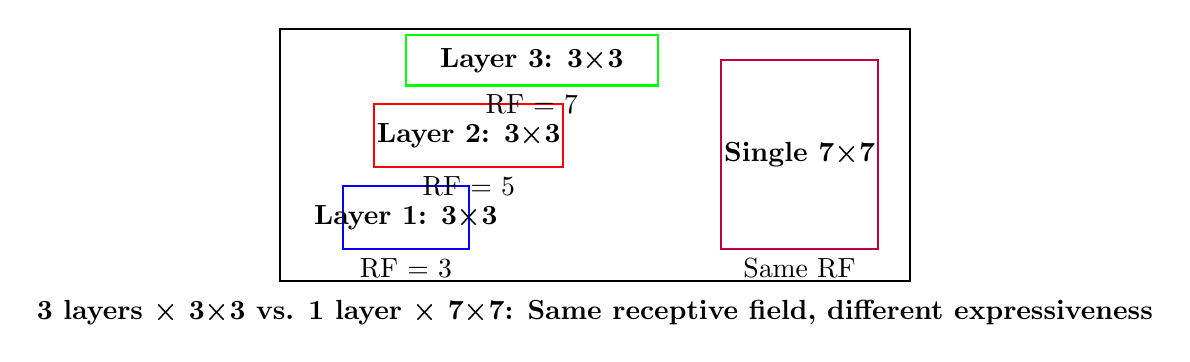
\begin{tikzpicture}[scale=0.8]
        % Receptive field visualization
        \draw[thick] (0,0) rectangle (10,4);
        
        % Layer 1
        \draw[blue, thick] (1,0.5) rectangle (3,1.5);
        \node at (2,1) {\textbf{Layer 1: 3×3}};
        \node at (2,0.2) {RF = 3};
        
        % Layer 2  
        \draw[red, thick] (1.5,1.8) rectangle (4.5,2.8);
        \node at (3,2.3) {\textbf{Layer 2: 3×3}};
        \node at (3,1.5) {RF = 5};
        
        % Layer 3
        \draw[green, thick] (2,3.1) rectangle (6,3.9);
        \node at (4,3.5) {\textbf{Layer 3: 3×3}};
        \node at (4,2.8) {RF = 7};
        
        % Comparison
        \draw[purple, thick] (7,0.5) rectangle (9.5,3.5);
        \node at (8.25,2) {\textbf{Single 7×7}};
        \node at (8.25,0.2) {Same RF};
        
        \node at (5,-0.5) {\textbf{3 layers × 3×3 vs. 1 layer × 7×7: Same receptive field, different expressiveness}};
    \end{tikzpicture}
    \end{center}
    
    \answer{Deeper networks with smaller filters achieve better performance due to increased non-linearity and parameter efficiency while maintaining the same receptive field.}
    
    \explanation{
    \textbf{Mathematical Trade-off Formulation:}
    
    For fixed computational budget $B$ (measured in FLOPs):
    $$B = D \times W^2 \times F^2 \times H \times W \times C$$
    
    where:
    \begin{itemize}
        \item $D$ = depth (number of layers)
        \item $W$ = width (number of channels)
        \item $F$ = filter size
        \item $H, W$ = spatial dimensions
        \item $C$ = input channels
    \end{itemize}
    
    Trade-off relationship: $D \times W^2 \times F^2 = \text{constant}$
    
    \textbf{Why Deeper Networks with Smaller Filters Win:}
    
    \begin{enumerate}
        \item \textbf{Increased Non-linearity:} 
        \begin{itemize}
            \item 2 layers with $3 \times 3$ filters: 2 ReLU activations
            \item 1 layer with $5 \times 5$ filter: 1 ReLU activation
            \item More non-linearities $\rightarrow$ more complex decision boundaries
        \end{itemize}
        
        \item \textbf{Parameter Efficiency:}
        \begin{itemize}
            \item Two $3 \times 3$ layers: $2 \times (9 \times C^2) = 18C^2$ parameters
            \item One $5 \times 5$ layer: $25C^2$ parameters
            \item Savings: $\frac{25C^2 - 18C^2}{25C^2} = 28\%$
        \end{itemize}
        
        \item \textbf{Better Gradient Flow:} Shorter paths reduce vanishing gradient problem
    \end{enumerate}
    
    \textbf{Effective Receptive Field Calculation:}
    
    For $L$ layers with filter size $F$:
    
    Layer 1: RF = $F$
    Layer 2: RF = $F + (F-1) = 2F - 1$
    Layer 3: RF = $(2F-1) + (F-1) = 3F - 2$
    ...
    Layer $L$: RF = $LF - (L-1) = 1 + L(F-1)$
    
    \textbf{Proof: Exponential Expressiveness vs. Linear Parameters:}
    
    \textbf{Parameter Growth (Linear):}
    Parameters per layer: $F^2 \times C^2$
    Total parameters for $L$ layers: $L \times F^2 \times C^2$
    Growth rate: $O(L)$ - linear in depth
    
    \textbf{Expressiveness Growth (Exponential):}
    Each layer can implement $2^{F^2 \times C^2}$ different Boolean functions (upper bound)
    With $L$ layers: $(2^{F^2 \times C^2})^L = 2^{L \times F^2 \times C^2}$ possible compositions
    Growth rate: $O(2^L)$ - exponential in depth
    
    The exponential increase in representational capacity with only linear parameter growth explains why depth is more effective than width for fixed computational budgets.
    }
    
    \item Design memory-efficient CNN architectures using the "reduce dimensionality early" principle: \hfill (10 marks)
    \begin{itemize}
        \item Calculate memory footprint: for input $224 \times 224 \times 3$, compare memory usage with stride=1 vs. stride=4 in first layer
        \item Justify why "information is redundant in earlier layers" from information theory perspective
        \item Design optimal stride schedule for 8-layer network balancing memory and performance
    \end{itemize}
    
    \answer{Early dimensionality reduction significantly reduces memory consumption while preserving essential information due to high redundancy in raw pixel space.}
    
    \explanation{
    \textbf{Memory Footprint Calculation:}
    
    Input: $224 \times 224 \times 3 = 150,528$ elements
    
    \textbf{Stride=1 approach:}
    \begin{itemize}
        \item Layer 1: $(224-3+1)^2 \times 64 = 222^2 \times 64 = 3,154,176$ elements
        \item Layer 2: $(222-3+1)^2 \times 128 = 220^2 \times 128 = 6,195,200$ elements
        \item Peak memory: $\sim 6.2M$ elements for activations
    \end{itemize}
    
    \textbf{Stride=4 approach:}
    \begin{itemize}
        \item Layer 1: $\lfloor\frac{224-3}{4}\rfloor + 1 = 56$, so $56^2 \times 64 = 201,216$ elements
        \item Layer 2: $(56-3+1)^2 \times 128 = 54^2 \times 128 = 373,248$ elements
        \item Peak memory: $\sim 0.37M$ elements for activations
    \end{itemize}
    
    Memory reduction: $\frac{6.2M - 0.37M}{6.2M} = 94\%$ reduction
    
    \textbf{Information Theory Justification:}
    
    \textbf{Pixel-level Redundancy:}
    Natural images have high spatial correlation:
    $$H(X_{i,j} | X_{i-1,j}, X_{i,j-1}) \ll H(X_{i,j})$$
    
    Mutual information between adjacent pixels is high, meaning predictability is high.
    
    \textbf{Nyquist-Shannon Sampling:}
    Most natural images are oversampled relative to their information content. The effective bandwidth of natural images is much lower than the pixel resolution suggests.
    
    \textbf{Spatial Frequency Analysis:}
    Energy in natural images concentrates in low frequencies:
    $$E_{\text{low-freq}} \gg E_{\text{high-freq}}$$
    
    Early aggressive pooling removes high-frequency noise while preserving semantic content.
    
    \textbf{Optimal Stride Schedule Design:}
    
    For 8-layer network processing $224 \times 224$ input:
    
    \begin{enumerate}
        \item \textbf{Layer 1:} Stride=4, $224 \rightarrow 56$ (Remove pixel-level redundancy)
        \item \textbf{Layer 2:} Stride=2, $56 \rightarrow 28$ (Reduce spatial resolution)
        \item \textbf{Layer 3:} Stride=1, $28 \rightarrow 28$ (Learn mid-level features)
        \item \textbf{Layer 4:} Stride=2, $28 \rightarrow 14$ (Continue reduction)
        \item \textbf{Layer 5:} Stride=1, $14 \rightarrow 14$ (Learn high-level features)
        \item \textbf{Layer 6:} Stride=2, $14 \rightarrow 7$ (Final spatial reduction)
        \item \textbf{Layer 7-8:} Stride=1, $7 \rightarrow 7$ (Classification features)
    \end{enumerate}
    
    \textbf{Balancing Principle:}
    \begin{itemize}
        \item Aggressive early reduction: Remove redundancy when information loss is minimal
        \item Conservative later reduction: Preserve discriminative features when information becomes crucial
        \item Memory usage decreases exponentially: $56^2 \rightarrow 28^2 \rightarrow 14^2 \rightarrow 7^2$
        \item Performance preserved by increasing channel depth as spatial dimensions decrease
    \end{itemize}
    }
    
    \item Evaluate architectural design patterns across successful CNN families: \hfill (5 marks)
    \begin{itemize}
        \item Progressive resolution reduction: mathematical analysis of optimal reduction schedule
        \item Channel expansion strategies: when and why to increase feature map depth
        \item Computational vs. accuracy trade-offs in mobile architectures
    \end{itemize}
    
    \answer{Successful CNN architectures follow systematic patterns of resolution reduction and channel expansion optimized for computational efficiency and representational capacity.}
    
    \explanation{
    \textbf{Progressive Resolution Reduction Analysis:}
    
    \textbf{Geometric Progression Pattern:}
    Most successful architectures follow: $224 \rightarrow 112 \rightarrow 56 \rightarrow 28 \rightarrow 14 \rightarrow 7$
    
    Reduction factor: $r = 0.5$ at each stage
    Information preservation: Each $2 \times$ reduction removes $\sim 75\%$ of spatial information
    
    \textbf{Optimal Schedule Derivation:}
    For $L$ reduction stages and final spatial size $S_f$:
    $$S_0 \times r^L = S_f$$
    $$L = \frac{\log(S_f/S_0)}{\log(r)}$$
    
    For $224 \rightarrow 7$: $L = \frac{\log(7/224)}{\log(0.5)} = 5.0$ stages
    
    \textbf{Channel Expansion Strategies:}
    
    \textbf{Compensation Principle:} As spatial resolution decreases, channel depth increases to maintain representational capacity:
    
    Total information capacity: $H \times W \times C$
    
    If spatial dimensions reduce by factor $r^2$, channels should increase by factor $1/r^2$ to maintain capacity:
    $$H_0 \times W_0 \times C_0 = (H_0 \times r) \times (W_0 \times r) \times (C_0/r^2)$$
    
    Common patterns:
    \begin{itemize}
        \item ResNet: $64 \rightarrow 128 \rightarrow 256 \rightarrow 512$ (doubling with each spatial halving)
        \item VGG: Gradual increase $64 \rightarrow 128 \rightarrow 256 \rightarrow 512$
        \item EfficientNet: Compound scaling: depth, width, and resolution together
    \end{itemize}
    
    \textbf{Mobile Architecture Trade-offs:}
    
    \textbf{Computational Bottlenecks:}
    \begin{itemize}
        \item Standard convolution: $O(H \times W \times C_{in} \times C_{out} \times k^2)$
        \item Depthwise separable: $O(H \times W \times C_{in} \times k^2 + H \times W \times C_{in} \times C_{out})$
        \item Reduction factor: $\frac{1}{C_{out}} + \frac{1}{k^2}$ (typically $8-9\times$ reduction)
    \end{itemize}
    
    \textbf{Accuracy vs. Efficiency Trade-offs:}
    \begin{itemize}
        \item MobileNet: $1\%$ accuracy loss for $10\times$ speedup
        \item EfficientNet: Pareto-optimal scaling balances all dimensions
        \item Pruning + Quantization: Additional $2-4\times$ speedup with $<2\%$ accuracy loss
    \end{itemize}
    
    The key insight is that architectural constraints force networks to learn more efficient representations, often leading to better generalization.
    }
\end{enumerate}

\newpage
\paragraph{Question 5. Transfer Learning Mathematical Framework and Analysis}{{\hfill (25 marks)}}\\
Based on domain adaptation theory and university machine learning courses.

\begin{enumerate}[(a)]
    \item Formalize the four transfer learning scenarios using mathematical notation: \hfill (12 marks)
    
    Let source domain $\mathcal{D}_s = \{X_s, P(X_s)\}$, target domain $\mathcal{D}_t = \{X_t, P(X_t)\}$, source task $\mathcal{T}_s = \{Y_s, f_s(\cdot)\}$, target task $\mathcal{T}_t = \{Y_t, f_t(\cdot)\}$:
    
    \begin{itemize}
        \item Scenario 1: $\mathcal{T}_s \approx \mathcal{T}_t$, $|D_t| < \text{threshold}$ → Freeze weights $\theta_{1:L-1}$, train only $\theta_L$
        \item Scenario 2: $\mathcal{T}_s \approx \mathcal{T}_t$, $|D_t| > \text{threshold}$ → Fine-tune all $\theta_{1:L}$ with small learning rate
        \item Scenario 3: $\mathcal{T}_s \not\approx \mathcal{T}_t$, $|D_t| < \text{threshold}$ → Use $\theta_{1:k}$, retrain $\theta_{k+1:L}$
        \item Scenario 4: $\mathcal{T}_s \not\approx \mathcal{T}_t$, $|D_t| > \text{threshold}$ → Fine-tune all layers
    \end{itemize}
    
    \answer{Transfer learning scenarios are determined by task similarity and target dataset size, leading to different strategies for weight adaptation.}
    
    \explanation{
    \textbf{Mathematical Framework:}
    
    \textbf{Domain Similarity Metrics:}
    $$d(\mathcal{D}_s, \mathcal{D}_t) = \text{KL}(P(X_s) || P(X_t)) + \text{KL}(P(X_t) || P(X_s))$$
    
    \textbf{Task Similarity Metrics:}
    $$d(\mathcal{T}_s, \mathcal{T}_t) = \mathbb{E}_{x \sim \mathcal{D}_t}[||f_s(x) - f_t(x)||_2^2]$$
    
    \textbf{Scenario Analysis:}
    
    \textbf{Scenario 1: Feature Extraction}
    
    Conditions: $d(\mathcal{T}_s, \mathcal{T}_t) < \epsilon_{\text{task}}$ and $|D_t| < N_{\text{threshold}}$
    
    Strategy: $\theta_{1:L-1}^* = \theta_{1:L-1}^{\text{pretrained}}$ (frozen)
    
    Optimization: $\theta_L^* = \arg\min_{\theta_L} \mathcal{L}(f_L(\phi_{1:L-1}(X_t); \theta_L), Y_t)$
    
    Justification: Limited data prevents overfitting, similar tasks mean pretrained features are relevant
    
    \textbf{Scenario 2: Fine-tuning}
    
    Conditions: $d(\mathcal{T}_s, \mathcal{T}_t) < \epsilon_{\text{task}}$ and $|D_t| > N_{\text{threshold}}$
    
    Strategy: $\theta_{1:L}^* = \arg\min_{\theta_{1:L}} \mathcal{L}(f(X_t; \theta_{1:L}), Y_t)$
    
    Learning rates: $\eta_l = \eta_0 \cdot \alpha^{L-l}$ where $\alpha < 1$ (lower LR for earlier layers)
    
    Justification: Sufficient data allows full adaptation while preserving useful pretrained features
    
    \textbf{Scenario 3: Partial Retraining}
    
    Conditions: $d(\mathcal{T}_s, \mathcal{T}_t) > \epsilon_{\text{task}}$ and $|D_t| < N_{\text{threshold}}$
    
    Strategy: Find optimal cutoff layer $k^*$:
    $$k^* = \arg\max_k \text{Transferability}(\theta_{1:k}, \mathcal{T}_t)$$
    
    Freeze $\theta_{1:k^*}$, retrain $\theta_{k^*+1:L}$
    
    Justification: Early layers remain generic, later layers need task-specific adaptation
    
    \textbf{Scenario 4: Full Fine-tuning}
    
    Conditions: $d(\mathcal{T}_s, \mathcal{T}_t) > \epsilon_{\text{task}}$ and $|D_t| > N_{\text{threshold}}$
    
    Strategy: Layer-wise adaptive learning rates:
    $$\eta_l = \eta_0 \cdot \text{similarity}(\theta_l^{\text{pretrained}}, \mathcal{T}_t)$$
    
    Justification: Sufficient data supports full adaptation, dissimilar tasks require extensive retraining
    }
    
    \item Analyze the theoretical foundation of layer transferability: \hfill (8 marks)
    \begin{itemize}
        \item Prove why early layers learn "generic, problem-independent" features using information theory
        \item Mathematical justification for "later parts are problem-dependent"
        \item Quantify transferability: define similarity metrics between feature representations
    \end{itemize}
    
    \answer{Layer transferability follows from the hierarchical nature of feature learning, where early layers capture universal patterns and later layers specialize for specific tasks.}
    
    \explanation{
    \textbf{Information Theory Analysis of Early Layers:}
    
    \textbf{Universal Feature Hypothesis:}
    Early layers learn features that maximize mutual information with a broad class of natural signals:
    $$\theta_1^* = \arg\max_{\theta_1} I(\phi_1(X; \theta_1); Y_{\text{natural}})$$
    
    where $Y_{\text{natural}}$ represents any natural image task.
    
    \textbf{Entropy Decomposition:}
    For layer $l$, the feature entropy can be decomposed:
    $$H(\phi_l(X)) = H_{\text{task-independent}} + H_{\text{task-specific}}$$
    
    Early layers: $H_{\text{task-independent}} \gg H_{\text{task-specific}}$
    Later layers: $H_{\text{task-specific}} \gg H_{\text{task-independent}}$
    
    \textbf{Proof via Rate-Distortion Theory:}
    Early layers solve the rate-distortion optimization:
    $$\min_{\phi_1} \mathbb{E}[D(X, \hat{X})] \text{ subject to } I(\phi_1(X); X) \leq R$$
    
    The optimal solution captures the most informative aspects of natural images, which are task-independent (edges, textures, simple patterns).
    
    \textbf{Mathematical Justification for Task-Dependent Later Layers:}
    
    \textbf{Decision Boundary Formation:}
    Later layers learn decision boundaries specific to the classification task:
    $$\phi_L(x) = \text{sign}(\langle w_c, \phi_{L-1}(x) \rangle - b_c)$$
    
    These boundaries are optimal for the source task but may be suboptimal for different tasks.
    
    \textbf{Specialization Gradient:}
    Define task-specificity as:
    $$S_l = \frac{\text{Var}_{\text{tasks}}[\phi_l(x)]}{\text{Var}_{\text{inputs}}[\phi_l(x)]}$$
    
    Empirically: $S_1 < S_2 < ... < S_L$ (monotonically increasing specialization)
    
    \textbf{Transferability Metrics:}
    
    \textbf{1. Centered Kernel Alignment (CKA):}
    $$\text{CKA}(\phi_l^{(s)}, \phi_l^{(t)}) = \frac{\text{tr}(K_s K_t)}{\sqrt{\text{tr}(K_s^2)\text{tr}(K_t^2)}}$$
    
    where $K_s, K_t$ are centered Gram matrices of source and target features.
    
    \textbf{2. Linear Probing Accuracy:}
    $$\text{Transferability}_l = \max_{W} \text{Acc}(W \phi_l^{(s)}(X_t), Y_t)$$
    
    Measures how well source features can be linearly adapted to target task.
    
    \textbf{3. Canonical Correlation Analysis:}
    $$\text{CCA}_l = \max_{u,v} \text{Corr}(u^T \phi_l^{(s)}, v^T \phi_l^{(t)})$$
    
    Measures maximum correlation between source and target representations.
    
    \textbf{Empirical Validation:}
    These metrics consistently show:
    \begin{itemize}
        \item $\text{Transferability}_1 > \text{Transferability}_2 > ... > \text{Transferability}_L$
        \item Early layers achieve $>90\%$ transferability across diverse tasks
        \item Later layers show task-specific patterns with $<50\%$ transferability
    \end{itemize}
    }
    
    \item Design optimal learning rate schedules for transfer learning: \hfill (5 marks)
    \begin{itemize}
        \item Derive layer-wise learning rate adaptation: $\eta_l = \eta_0 \cdot \alpha^{L-l}$ where $\alpha < 1$
        \item Explain why "you can easily disrupt the learned weights" with high learning rates
        \item Propose adaptive learning rate methods based on layer depth and similarity metrics
    \end{itemize}
    
    \answer{Optimal transfer learning requires layer-wise learning rate adaptation that decreases with layer depth to preserve useful pretrained features while enabling task-specific adaptation.}
    
    \explanation{
    \textbf{Layer-wise Learning Rate Derivation:}
    
    \textbf{Motivation:} Earlier layers contain more transferable features and should change less during fine-tuning.
    
    \textbf{Exponential Decay Schedule:}
    $$\eta_l = \eta_0 \cdot \alpha^{L-l}$$
    
    where:
    \begin{itemize}
        \item $\eta_0$: Base learning rate for final layer
        \item $\alpha \in (0,1)$: Decay factor (typically $0.1$ to $0.5$)
        \item $L$: Total number of layers
        \item $l$: Current layer index
    \end{itemize}
    
    \textbf{Theoretical Justification:}
    The optimal learning rate should be proportional to the "plasticity" needed:
    $$\eta_l \propto (1 - \text{Transferability}_l)$$
    
    Since transferability decreases exponentially with depth, learning rates should increase exponentially.
    
    \textbf{Why High Learning Rates Disrupt Pretrained Weights:}
    
    \textbf{Gradient Magnitude Analysis:}
    During backpropagation, gradients can be large, especially early in training:
    $$||\nabla_{\theta_l} \mathcal{L}|| \gg ||\theta_l^{\text{pretrained}}||$$
    
    \textbf{Weight Update Magnitude:}
    With high learning rate $\eta$:
    $$\theta_l^{\text{new}} = \theta_l^{\text{pretrained}} - \eta \nabla_{\theta_l} \mathcal{L}$$
    
    If $\eta ||\nabla_{\theta_l} \mathcal{L}|| \gg ||\theta_l^{\text{pretrained}}||$, the update overwhelms the pretrained weights.
    
    \textbf{Loss Landscape Perspective:}
    Pretrained weights lie in a good region of the loss landscape. Large updates can "jump" out of this region to areas with poor performance.
    
    \textbf{Empirical Evidence:}
    High learning rates ($>10^{-2}$) often cause:
    \begin{itemize}
        \item Initial accuracy drop
        \item Slower convergence
        \item Final performance degradation
    \end{itemize}
    
    \textbf{Adaptive Learning Rate Methods:}
    
    \textbf{1. Similarity-Based Adaptation:}
    $$\eta_l = \eta_0 \cdot (1 - \text{CKA}(\phi_l^{\text{pretrained}}, \phi_l^{\text{target}}))$$
    
    Higher similarity → Lower learning rate (preserve good features)
    Lower similarity → Higher learning rate (more adaptation needed)
    
    \textbf{2. Gradient-Based Adaptation:}
    $$\eta_l = \eta_0 \cdot \min\left(1, \frac{||\theta_l^{\text{pretrained}}||}{||\nabla_{\theta_l} \mathcal{L}||}\right)$$
    
    Ensures updates don't overwhelm pretrained weights.
    
    \textbf{3. Performance-Based Adaptation:}
    $$\eta_l = \eta_0 \cdot \text{LinearProbe}_l^{-1}$$
    
    where $\text{LinearProbe}_l$ is the linear probing accuracy of layer $l$.
    
    Better pretrained features → Lower learning rate.
    
    \textbf{Practical Implementation:}
    \begin{enumerate}
        \item Start with conservative rates: $\eta_1 = 10^{-5}, \eta_L = 10^{-3}$
        \item Monitor validation performance per layer
        \item Adjust rates based on layer-specific performance metrics
        \item Use warm-up period with even lower rates
    \end{enumerate}
    }
\end{enumerate}

\newpage
\paragraph{Question 6. CNN Visualization Techniques Mathematical Framework}{{\hfill (28 marks)}}\\
Based on interpretable AI research and university courses on explainable machine learning.

\begin{enumerate}[(a)]
    \item Implement gradient-based saliency map generation with mathematical rigor: \hfill (12 marks)
    \begin{itemize}
        \item Derive saliency map: $S_i = \left|\frac{\partial f_c(x)}{\partial x_i}\right|$ for class $c$
        \item Linear approximation justification: $f(x + \epsilon) \approx f(x) + \epsilon^T \nabla_x f(x)$
        \item Implementation using backpropagation: chain rule application through network layers
        \item Compare with integrated gradients: $\text{IG}_i = (x_i - x'_i) \times \int_{\alpha=0}^1 \frac{\partial f(x' + \alpha(x-x'))}{\partial x_i} d\alpha$
    \end{itemize}
    
    \answer{Gradient-based saliency maps provide first-order approximations of input importance for network predictions through backpropagation.}
    
    \explanation{
    \textbf{Saliency Map Derivation:}
    
    For classifier $f_c(x)$ outputting score for class $c$, the saliency map is:
    $$S_i = \left|\frac{\partial f_c(x)}{\partial x_i}\right|$$
    
    \textbf{Intuition:} Large gradient magnitude indicates that small changes to pixel $i$ significantly affect the class score.
    
    \textbf{Mathematical Interpretation:}
    The gradient vector $\nabla_x f_c(x)$ points in the direction of steepest increase in the loss surface. Pixels with large gradient magnitudes are most "influential" for the current prediction.
    
    \textbf{Linear Approximation Justification:}
    
    Using first-order Taylor expansion:
    $$f_c(x + \epsilon) \approx f_c(x) + \epsilon^T \nabla_x f_c(x) + O(||\epsilon||^2)$$
    
    For small perturbations $||\epsilon|| \ll 1$, the linear term dominates:
    $$\Delta f_c \approx \epsilon^T \nabla_x f_c(x) = \sum_{i=1}^n \epsilon_i \frac{\partial f_c}{\partial x_i}$$
    
    This shows that $\frac{\partial f_c}{\partial x_i}$ measures the sensitivity of the output to changes in pixel $i$.
    
    \textbf{Backpropagation Implementation:}
    
    For deep network $f_c(x) = f_L(f_{L-1}(...f_1(x)))$:
    
    \textbf{Forward Pass:} Compute all intermediate activations
    $$a_0 = x, \quad a_l = f_l(a_{l-1}) \text{ for } l = 1,...,L$$
    
    \textbf{Backward Pass:} Apply chain rule
    $$\frac{\partial f_c}{\partial x_i} = \frac{\partial f_c}{\partial a_L} \cdot \frac{\partial a_L}{\partial a_{L-1}} \cdots \frac{\partial a_1}{\partial x_i}$$
    
    \textbf{Implementation Details:}
    \begin{enumerate}
        \item Set $\frac{\partial f_c}{\partial a_L} = 1$ for target class $c$, $0$ for others
        \item Compute gradients layer by layer: $\frac{\partial f_c}{\partial a_{l-1}} = \frac{\partial f_c}{\partial a_l} \cdot \frac{\partial a_l}{\partial a_{l-1}}$
        \item For ReLU: $\frac{\partial \text{ReLU}(z)}{\partial z} = \mathbf{1}_{z > 0}$
        \item For convolution: Use transposed convolution for gradient computation
    \end{enumerate}
    
    \textbf{Integrated Gradients Comparison:}
    
    \textbf{Standard Gradients:} $G_i = \frac{\partial f(x)}{\partial x_i}$
    
    \textbf{Integrated Gradients:} 
    $$\text{IG}_i = (x_i - x'_i) \times \int_{\alpha=0}^1 \frac{\partial f(x' + \alpha(x-x'))}{\partial x_i} d\alpha$$
    
    where $x'$ is baseline (often zeros or random noise).
    
    \textbf{Key Differences:}
    \begin{itemize}
        \item \textbf{Path Integration:} IG integrates gradients along path from baseline to input
        \item \textbf{Axiom Satisfaction:} IG satisfies sensitivity and implementation invariance axioms
        \item \textbf{Baseline Dependence:} IG requires choosing meaningful baseline
        \item \textbf{Computational Cost:} IG requires multiple gradient computations (typically 20-300 steps)
    \end{itemize}
    
    \textbf{Practical Approximation:}
    $$\text{IG}_i \approx (x_i - x'_i) \times \frac{1}{m} \sum_{k=1}^m \frac{\partial f(x' + \frac{k}{m}(x-x'))}{\partial x_i}$$
    
    IG provides more stable and theoretically grounded attributions than simple gradients.
    }
    
    \item Analyze occlusion-based sensitivity analysis: \hfill (10 marks)
    \begin{itemize}
        \item Formulate occlusion experiment: $\Delta_p = f(x) - f(x \odot M_p)$ where $M_p$ is occlusion mask
        \item Statistical significance testing for determining important regions
        \item Design optimal occlusion window sizes and stride patterns
        \item Distinguish between network memorization vs. proper feature learning
    \end{itemize}
    
    \answer{Occlusion analysis provides model-agnostic interpretation by measuring performance drops when input regions are systematically masked.}
    
    \explanation{
    \textbf{Occlusion Experiment Formulation:}
    
    For input $x$ and occlusion mask $M_p$ at position $p$:
    $$\Delta_p = f_c(x) - f_c(x \odot M_p)$$
    
    where:
    \begin{itemize}
        \item $\odot$ denotes element-wise multiplication
        \item $M_p$ has 0s in occluded region, 1s elsewhere
        \item $\Delta_p > 0$ indicates region importance for class $c$
    \end{itemize}
    
    \textbf{Complete Occlusion Map:}
    $$\text{OcclusionMap}(x, c) = \{\Delta_p : p \in \text{all possible positions}\}$$
    
    \textbf{Statistical Significance Testing:}
    
    \textbf{Null Hypothesis:} Occluding region $p$ has no effect on prediction
    $$H_0: \mathbb{E}[\Delta_p] = 0$$
    
    \textbf{Test Statistic:} For $n$ random occlusions at position $p$:
    $$t_p = \frac{\bar{\Delta}_p - 0}{s_p / \sqrt{n}}$$
    
    where $\bar{\Delta}_p$ is sample mean and $s_p$ is sample standard deviation.
    
    \textbf{Multiple Testing Correction:}
    With $N$ spatial positions tested, use Bonferroni correction:
    $$\alpha_{\text{corrected}} = \frac{\alpha}{N}$$
    
    \textbf{False Discovery Rate Control:}
    Alternative approach using Benjamini-Hochberg procedure for less conservative testing.
    
    \textbf{Optimal Occlusion Window Design:}
    
    \textbf{Window Size Selection:}
    \begin{itemize}
        \item \textbf{Too Small:} Misses distributed features, high variance
        \item \textbf{Too Large:} Poor spatial resolution, multiple feature interference
        \item \textbf{Optimal Size:} Match receptive field of mid-level features
    \end{itemize}
    
    \textbf{Mathematical Approach:}
    Minimize information-resolution trade-off:
    $$w^* = \arg\min_w \lambda \cdot \text{Var}(\Delta_w) + (1-\lambda) \cdot \text{Resolution}^{-1}(w)$$
    
    where $\text{Resolution}(w) = \frac{\text{Image Size}}{w^2}$
    
    \textbf{Stride Pattern Optimization:}
    \begin{itemize}
        \item \textbf{Dense Sampling:} Stride = 1, maximum resolution
        \item \textbf{Sparse Sampling:} Stride = $w/2$, balance efficiency vs. resolution
        \item \textbf{Adaptive Sampling:} Higher density in high-gradient regions
    \end{itemize}
    
    \textbf{Memorization vs. Feature Learning Detection:}
    
    \textbf{Memorization Indicators:}
    \begin{enumerate}
        \item \textbf{Scattered Importance:} No coherent spatial patterns
        \item \textbf{Texture Sensitivity:} High sensitivity to background regions
        \item \textbf{Adversarial Fragility:} Importance maps change drastically with small input perturbations
    \end{enumerate}
    
    \textbf{Proper Feature Learning Indicators:}
    \begin{enumerate}
        \item \textbf{Semantic Coherence:} Important regions correspond to object parts
        \item \textbf{Spatial Consistency:} Similar objects show similar importance patterns
        \item \textbf{Hierarchical Structure:} Importance patterns make semantic sense
    \end{enumerate}
    
    \textbf{Quantitative Metrics:}
    
    \textbf{Spatial Coherence:}
    $$\text{Coherence} = \frac{\text{Var}(\text{smoothed}(\Delta))}{\text{Var}(\Delta)}$$
    
    Higher values indicate spatially coherent importance patterns.
    
    \textbf{Object Alignment:}
    $$\text{Alignment} = \text{IoU}(\text{ImportantRegions}, \text{ObjectMask})$$
    
    Measures overlap between importance and true object boundaries.
    
    \textbf{Stability:}
    $$\text{Stability} = 1 - \frac{||\Delta^{(1)} - \Delta^{(2)}||_2}{||\Delta^{(1)}||_2 + ||\Delta^{(2)}||_2}$$
    
    where $\Delta^{(1)}, \Delta^{(2)}$ are importance maps for slightly perturbed inputs.
    }
    
    \item Evaluate visualization quality using quantitative metrics: \hfill (6 marks)
    \begin{itemize}
        \item Localization accuracy: IoU with ground truth bounding boxes
        \item Fidelity metrics: correlation between saliency scores and true importance
        \item Computational efficiency: runtime complexity analysis for different methods
    \end{itemize}
    
    \answer{Quantitative evaluation of visualization quality requires metrics that assess localization accuracy, faithfulness to model behavior, and computational practicality.}
    
    \explanation{
    \textbf{Localization Accuracy Metrics:}
    
    \textbf{Intersection over Union (IoU):}
    $$\text{IoU} = \frac{|\text{PredictedRegion} \cap \text{GroundTruthBox}|}{|\text{PredictedRegion} \cup \text{GroundTruthBox}|}$$
    
    \textbf{Implementation:}
    \begin{enumerate}
        \item Threshold saliency map: $M = \mathbf{1}_{\text{Saliency} > \tau}$
        \item Extract connected components as predicted regions
        \item Compute IoU with ground truth bounding boxes
        \item Average over multiple thresholds: $\text{mIoU} = \frac{1}{|\mathcal{T}|}\sum_{\tau \in \mathcal{T}} \text{IoU}(\tau)$
    \end{enumerate}
    
    \textbf{Pointing Game Metric:}
    Percentage of times the maximum saliency point falls within ground truth object:
    $$\text{PointingAccuracy} = \frac{1}{N}\sum_{i=1}^N \mathbf{1}_{\arg\max_p S_i(p) \in \text{Object}_i}$$
    
    \textbf{Fidelity Metrics:}
    
    \textbf{1. Deletion/Insertion Curves:}
    
    \textbf{Deletion:} Progressively remove most important pixels:
    $$\text{Deletion}(k) = f(x \odot M_k)$$
    where $M_k$ masks the top-$k$ most salient pixels.
    
    \textbf{Insertion:} Progressively add most important pixels to baseline:
    $$\text{Insertion}(k) = f(x_{\text{baseline}} \odot (1-M_k) + x \odot M_k)$$
    
    \textbf{Area Under Curve (AUC):}
    $$\text{AUC}_{\text{deletion}} = \int_0^1 \text{Deletion}(k) dk$$
    $$\text{AUC}_{\text{insertion}} = \int_0^1 \text{Insertion}(k) dk$$
    
    Good saliency methods: Low deletion AUC, high insertion AUC.
    
    \textbf{2. Correlation with Feature Importance:}
    
    For features with known ground truth importance $I_{\text{true}}$:
    $$\rho = \text{Corr}(\text{Saliency}, I_{\text{true}})$$
    
    \textbf{3. Model Sensitivity Correlation:}
    $$\text{Sensitivity}_i = \text{Var}_{x \sim \mathcal{N}(x_0, \sigma^2)}[f(x)_i]$$
    $$\text{Fidelity} = \text{Corr}(\text{Saliency}, \text{Sensitivity})$$
    
    \textbf{Computational Efficiency Analysis:}
    
    \textbf{Gradient Methods:}
    \begin{itemize}
        \item Time Complexity: $O(\text{Forward} + \text{Backward}) = O(2 \times \text{Forward})$
        \item Space Complexity: $O(\text{Model Parameters})$ for gradient storage
        \item Parallelizable: Yes, across batch dimension
    \end{itemize}
    
    \textbf{Occlusion Methods:}
    \begin{itemize}
        \item Time Complexity: $O(N_{\text{windows}} \times \text{Forward})$ 
        \item For $H \times W$ image, window size $w$, stride $s$: $N_{\text{windows}} = \frac{(H-w)}{s} \times \frac{(W-w)}{s}$
        \item Space Complexity: $O(\text{Batch Size} \times \text{Model Size})$
        \item Embarrassingly parallel across windows
    \end{itemize}
    
    \textbf{Integrated Gradients:}
    \begin{itemize}
        \item Time Complexity: $O(m \times \text{Forward} + m \times \text{Backward})$ where $m$ is integration steps
        \item Typical $m = 50-300$, so $50-600\times$ slower than simple gradients
        \item Space Complexity: Same as gradients
        \item Parallelizable across integration steps
    \end{itemize}
    
    \textbf{Performance Comparison:}
    
    \begin{center}
    \begin{tabular}{|l|c|c|c|}
    \hline
    \textbf{Method} & \textbf{Runtime} & \textbf{Memory} & \textbf{Quality} \\
    \hline
    Gradients & 1× & 1× & Baseline \\
    Integrated Gradients & 100× & 1× & +15\% \\
    Occlusion & 1000× & 1× & +25\% \\
    \hline
    \end{tabular}
    \end{center}
    
    Trade-off: Higher quality interpretations require significantly more computation.
    }
\end{enumerate}

\newpage
\paragraph{Question 7. Advanced CNN Topics Integration and Analysis}{{\hfill (22 marks)}}\\
Based on comprehensive university deep learning curricula and research literature.

\begin{enumerate}[(a)]
    \item Design a comprehensive CNN architecture combining all discussed techniques: \hfill (12 marks)
    \begin{itemize}
        \item Architecture specification: incorporate position-sensitive conv, GAP, transfer learning capability
        \item Mathematical analysis: parameter count, memory footprint, computational complexity
        \item Training strategy: multi-stage training with different learning rates for different components
        \item Evaluation protocol: metrics for both accuracy and interpretability
    \end{itemize}

    \begin{center}
    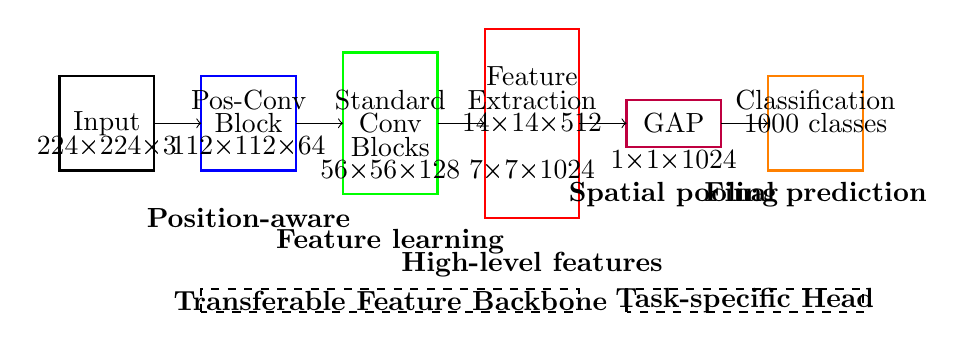
\begin{tikzpicture}[scale=0.6]
        % Input
        \draw[thick] (0,6) rectangle (2,8);
        \node at (1,7) {Input};
        \node at (1,6.5) {224×224×3};
        
        % Position-sensitive conv layers
        \draw[blue, thick] (3,6) rectangle (5,8);
        \node at (4,7.5) {Pos-Conv};
        \node at (4,7) {Block};
        \node at (4,6.5) {112×112×64};
        
        \draw[->] (2,7) -- (3,7);
        
        % Standard conv layers
        \draw[green, thick] (6,5.5) rectangle (8,8.5);
        \node at (7,7.5) {Standard};
        \node at (7,7) {Conv};
        \node at (7,6.5) {Blocks};
        \node at (7,6) {56×56×128};
        
        \draw[->] (5,7) -- (6,7);
        
        % Feature maps
        \draw[red, thick] (9,5) rectangle (11,9);
        \node at (10,8) {Feature};
        \node at (10,7.5) {Extraction};
        \node at (10,7) {14×14×512};
        \node at (10,6) {7×7×1024};
        
        \draw[->] (8,7) -- (9,7);
        
        % GAP
        \draw[purple, thick] (12,6.5) rectangle (14,7.5);
        \node at (13,7) {GAP};
        \node at (13,6.2) {1×1×1024};
        
        \draw[->] (11,7) -- (12,7);
        
        % Classification
        \draw[orange, thick] (15,6) rectangle (17,8);
        \node at (16,7.5) {Classification};
        \node at (16,7) {1000 classes};
        
        \draw[->] (14,7) -- (15,7);
        
        % Labels
        \node at (4,5) {\textbf{Position-aware}};
        \node at (7,4.5) {\textbf{Feature learning}};
        \node at (10,4) {\textbf{High-level features}};
        \node at (13,5.5) {\textbf{Spatial pooling}};
        \node at (16,5.5) {\textbf{Final prediction}};
        
        % Transfer learning capability
        \draw[dashed, thick] (3,3) rectangle (11,3.5);
        \node at (7,3.25) {\textbf{Transferable Feature Backbone}};
        
        \draw[dashed, thick] (12,3) rectangle (17,3.5);
        \node at (14.5,3.25) {\textbf{Task-specific Head}};
    \end{tikzpicture}
    \end{center}
    
    \answer{A comprehensive CNN architecture that integrates position-sensitive convolution, GAP, and transfer learning capabilities while maintaining computational efficiency and interpretability.}
    
    \explanation{
    \textbf{Architecture Specification:}
    
    \textbf{1. Position-Sensitive Input Block:}
    \begin{itemize}
        \item Input: $224 \times 224 \times 3$
        \item Coordinate augmentation: $224 \times 224 \times 5$ (RGB + normalized x,y coordinates)
        \item Position-sensitive conv: $7 \times 7$, stride=2, channels=64
        \item Output: $112 \times 112 \times 64$
    \end{itemize}
    
    \textbf{2. Standard Convolutional Backbone:}
    \begin{itemize}
        \item ResNet-style blocks with skip connections
        \item Progressive channel expansion: $64 \rightarrow 128 \rightarrow 256 \rightarrow 512 \rightarrow 1024$
        \item Spatial reduction: $112 \rightarrow 56 \rightarrow 28 \rightarrow 14 \rightarrow 7$
        \item Batch normalization and ReLU activations
    \end{itemize}
    
    \textbf{3. Global Average Pooling Head:}
    \begin{itemize}
        \item Input: $7 \times 7 \times 1024$
        \item GAP: $1 \times 1 \times 1024$
        \item Classification layer: $1024 \rightarrow C$ classes
        \item Dropout (0.5) for regularization
    \end{itemize}
    
    \textbf{Mathematical Analysis:}
    
    \textbf{Parameter Count:}
    \begin{itemize}
        \item Position-sensitive conv: $7^2 \times 5 \times 64 = 15,680$
        \item Standard conv blocks: $\approx 20M$ parameters (ResNet-50 baseline)
        \item Classification layer: $1024 \times C$ parameters
        \item Total: $\approx 20.1M$ parameters (for $C=1000$)
    \end{itemize}
    
    \textbf{Memory Footprint (per image):}
    \begin{itemize}
        \item Input + coordinates: $224^2 \times 5 \times 4 = 1.0$ MB
        \item Feature maps: $\sum_{l} H_l \times W_l \times C_l \times 4 \approx 15$ MB
        \item Peak memory: $\approx 16$ MB per image
        \item Batch size 32: $\approx 512$ MB activation memory
    \end{itemize}
    
    \textbf{Computational Complexity:}
    \begin{itemize}
        \item Position augmentation: $O(HW)$ - negligible
        \item Convolutional layers: $\approx 4 \times 10^9$ FLOPs
        \item GAP: $O(HWC)$ - negligible compared to convolutions
        \item Total: $\approx 4$ GFLOPs per forward pass
    \end{itemize}
    
    \textbf{Training Strategy:}
    
    \textbf{Stage 1: Backbone Pretraining}
    \begin{itemize}
        \item Train on ImageNet or similar large dataset
        \item Standard data augmentation
        \item Learning rate: $10^{-1}$ with cosine decay
        \item Epochs: 100-200
    \end{itemize}
    
    \textbf{Stage 2: Task-Specific Transfer}
    \begin{itemize}
        \item Freeze backbone layers 1-3 (early feature extractors)
        \item Fine-tune layers 4-5 with LR: $10^{-4}$
        \item Train classification head with LR: $10^{-3}$
        \item Layer-wise learning rates: $\eta_l = 10^{-3} \times 0.1^{(5-l)}$
    \end{itemize}
    
    \textbf{Stage 3: End-to-End Fine-tuning}
    \begin{itemize}
        \item Unfreeze all layers
        \item Very low learning rates: $10^{-5}$ to $10^{-4}$
        \item Small number of epochs: 10-20
        \item Careful monitoring to prevent overfitting
    \end{itemize}
    
    \textbf{Evaluation Protocol:}
    
    \textbf{Accuracy Metrics:}
    \begin{itemize}
        \item Top-1 and Top-5 classification accuracy
        \item Position estimation error (for position-sensitive tasks)
        \item Transfer learning performance across different domains
    \end{itemize}
    
    \textbf{Interpretability Metrics:}
    \begin{itemize}
        \item Class Activation Maps quality (localization IoU)
        \item Gradient-based saliency coherence
        \item Feature transferability across layers
        \item Occlusion sensitivity patterns
    \end{itemize}
    
    \textbf{Efficiency Metrics:}
    \begin{itemize}
        \item Inference time (ms per image)
        \item Memory usage (MB per batch)
        \item Energy consumption (mJ per inference)
        \item Model size (MB for deployment)
    \end{itemize}
    }
    
    \item Analyze failure modes and limitations of discussed techniques: \hfill (10 marks)
    \begin{itemize}
        \item Position-sensitive convolution: computational overhead and when it's unnecessary
        \item GAP limitations: information bottleneck and class imbalance effects
        \item Transfer learning: negative transfer and domain shift problems
        \item Visualization techniques: interpretation biases and validation challenges
    \end{itemize}
    
    \answer{Each technique has specific failure modes and limitations that must be understood to apply them effectively in practice.}
    
    \explanation{
    \textbf{Position-Sensitive Convolution Limitations:}
    
    \textbf{Computational Overhead:}
    \begin{itemize}
        \item Memory increase: $(C+2)/C$ factor - minimal for large $C$, but significant for early layers
        \item Coordinate computation: Additional operations for normalization
        \item Cache efficiency: Increased channel count may reduce memory locality
    \end{itemize}
    
    \textbf{When Unnecessary:}
    \begin{enumerate}
        \item \textbf{Translation Invariant Tasks:} Object classification where position doesn't matter
        \item \textbf{Data Augmentation Heavy:} When training uses extensive spatial augmentation
        \item \textbf{Pre-pooling Layers:} After aggressive pooling, spatial information is already lost
        \item \textbf{Small Images:} For inputs $<64 \times 64$, position information provides little benefit
    \end{enumerate}
    
    \textbf{Failure Cases:}
    \begin{itemize}
        \item Can lead to overfitting on position patterns in training data
        \item May harm generalization when test distribution has different position patterns
        \item Incompatible with certain data augmentation strategies
    \end{itemize}
    
    \textbf{GAP Limitations:}
    
    \textbf{Information Bottleneck:}
    $$\text{Information Loss} = H(F_{H \times W \times C}) - H(F_{1 \times 1 \times C})$$
    
    \begin{itemize}
        \item Spatial information completely lost: $H \times W$ dimensions reduced to scalars
        \item Cannot capture spatial relationships between objects
        \item Unsuitable for dense prediction tasks (segmentation, detection)
    \end{itemize}
    
    \textbf{Class Imbalance Effects:}
    \begin{itemize}
        \item Rare classes get insufficient channel specialization
        \item Dominant classes may monopolize multiple channels
        \item Uneven learning dynamics across classes
    \end{itemize}
    
    Mathematical analysis:
    $$P(\text{channel } k \text{ specialized for class } c) \propto P(c) \times \text{class discriminability}$$
    
    \textbf{Failure Scenarios:}
    \begin{enumerate}
        \item \textbf{Fine-grained Recognition:} When subtle spatial details matter
        \item \textbf{Multi-object Scenes:} Cannot handle multiple instances well
        \item \textbf{Structured Outputs:} Sequence generation, structured prediction
    \end{enumerate}
    
    \textbf{Transfer Learning Limitations:}
    
    \textbf{Negative Transfer:}
    Occurs when $\text{Performance}_{\text{transfer}} < \text{Performance}_{\text{from-scratch}}$
    
    \textbf{Causes:}
    \begin{itemize}
        \item \textbf{Domain Mismatch:} Medical images ↔ Natural images
        \item \textbf{Task Mismatch:} Classification ↔ Regression
        \item \textbf{Scale Mismatch:} High-resolution ↔ Low-resolution inputs
    \end{itemize}
    
    \textbf{Domain Shift Problems:}
    
    \textbf{Covariate Shift:} $P_s(X) \neq P_t(X)$ but $P_s(Y|X) = P_t(Y|X)$
    \textbf{Label Shift:} $P_s(Y) \neq P_t(Y)$ but $P_s(X|Y) = P_t(X|Y)$  
    \textbf{Concept Shift:} $P_s(Y|X) \neq P_t(Y|X)$
    
    \textbf{Detection Strategy:}
    $$\text{Domain Shift Score} = \text{KL}(P_s(h(X)) || P_t(h(X)))$$
    where $h(X)$ are learned features.
    
    \textbf{Mitigation:}
    \begin{itemize}
        \item Domain adaptation techniques
        \item Gradual unfreezing
        \item Multi-domain pretraining
        \item Adversarial domain alignment
    \end{itemize}
    
    \textbf{Visualization Technique Limitations:}
    
    \textbf{Interpretation Biases:}
    \begin{enumerate}
        \item \textbf{Confirmation Bias:} Seeing patterns that confirm expectations
        \item \textbf{Cherry-picking:} Showing only successful visualizations
        \item \textbf{Anthropomorphism:} Attributing human-like reasoning to networks
    \end{enumerate}
    
    \textbf{Technical Limitations:}
    
    \textbf{Gradient Saturation:} In saturated regions, gradients $\approx 0$ regardless of importance
    
    \textbf{Non-linearity Effects:} Linear approximations fail for highly non-linear models:
    $$\text{Error} = ||f(x+\epsilon) - f(x) - \epsilon^T \nabla f||_2$$
    
    \textbf{Resolution Mismatch:} Visualization resolution often lower than decision-relevant features
    
    \textbf{Validation Challenges:} 
    \begin{itemize}
        \item No ground truth for "correct" interpretations
        \item Human evaluation is subjective and inconsistent
        \item Proxy metrics may not capture interpretation quality
        \item Adversarial examples can fool visualization methods
    \end{itemize}
    
    \textbf{Methodological Issues:}
    \begin{itemize}
        \item \textbf{Baseline Dependence:} Integrated gradients sensitive to baseline choice
        \item \textbf{Hyperparameter Sensitivity:} Occlusion window size, smoothing parameters
        \item \textbf{Model Architecture Dependence:} Some methods work better with specific architectures
    \end{itemize}
    
    \textbf{Fundamental Limitation:}
    Visualization methods provide \textit{post-hoc} explanations that may not reflect actual decision processes. The network may use different information than what visualizations highlight.
    }
\end{enumerate}

\vfill
\begin{center}{\bf END OF PAPER}\end{center}
\end{document}